\newpage
\section{Kolejne wersje programu}

Program nie powstał od razu w docelowej postaci. Każda iteracja dokładała jeden brak, który wychodził przy próbie uruchomienia poprzedniej wersji na obiekcie zbliżonym do rzeczywistej linii.

\subsection{Rozruch od przełącznika}

Na początku założyliśmy, że START jest przełącznikiem bistabilnym podanym stale na I1. Dopóki na I1 jest jedynka, linia ma pracować. Zdjęcie sygnału gasi wszystko.

W pierwszych dwóch szczeblach sygnał I1 jednocześnie uruchamia timer T1 i załącza napęd 1 na Q1. Nic więcej się nie dzieje, dopóki T1 nie odmierzy nastawy. Po tym czasie startuje T2 i równolegle napęd 2 na Q2. Gdy skończy się T2, załącza się napęd 3 na Q3. Trzy silniki ruszają więc po kolei, z przerwami równymi nastawom timerów. Zanik I1 w dowolnym momencie zeruje wyjścia i kasuje timery, bo całe drzewo warunków wisi na tym jednym sygnale.

\begin{figure}[H]
    \centering
    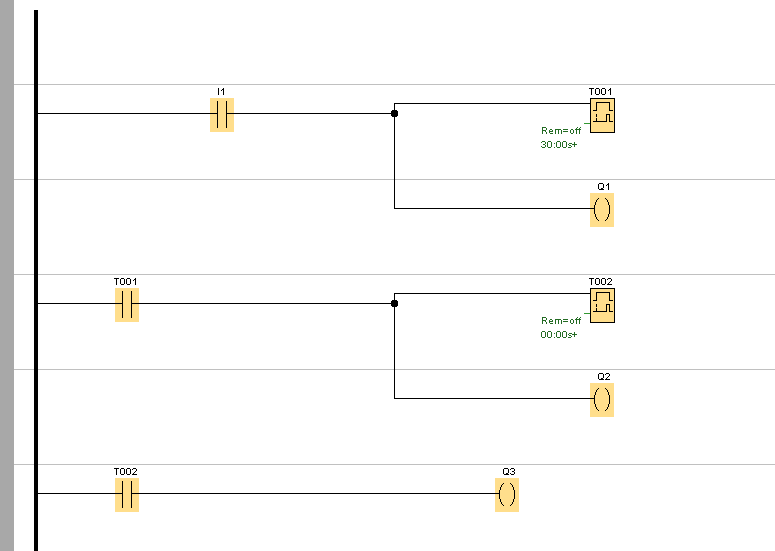
\includegraphics[width=0.92\textwidth]{rys/iteracja1.png}
    \caption{Iteracja 1 --- START ciągły i dwa timery}
    \label{fig:iter1}
\end{figure}

Taki układ da się zasymulować i czasy zgadzają się z nastawami, ale jako sterowanie linii jest ryzykowny. Po zaniku napięcia sterownik wstaje z programem, a jeśli przełącznik START został w pozycji załączonej, taśmociągi ruszają same. Tego właśnie chcieliśmy uniknąć w następnym kroku.

\subsection{Przyciski START i STOP oraz marker}

START przenieśliśmy na przycisk monostabilny (I1), a zatrzymanie na osobny przycisk (I2). Stan „linia pracuje” trzyma marker M1.

W pierwszym cyklu sterownik widzi zanegowany STOP. Przy I2 równym zero styk przepuszcza sygnał dalej. Jeśli w tym samym szczeblu pojawi się jedynka na I1, cewka M1 zostaje ustawiona. W kolejnym cyklu przycisk START jest już puszczony, ale drugi szczebel czyta M1 i tym samym stykiem podtrzymuje cewkę. Naciśnięcie STOP odwraca warunek na początku szeregu i marker odpada niezależnie od I1 oraz od własnego podtrzymania.

Od trzeciego szczebla reszta programu jest ta sama co w pierwszej wersji, tylko zamiast surowego I1 steruje nią M1. Po powrocie zasilania marker jest zgaszony, więc linia czeka na ponowne wciśnięcie START.

\begin{figure}[H]
    \centering
    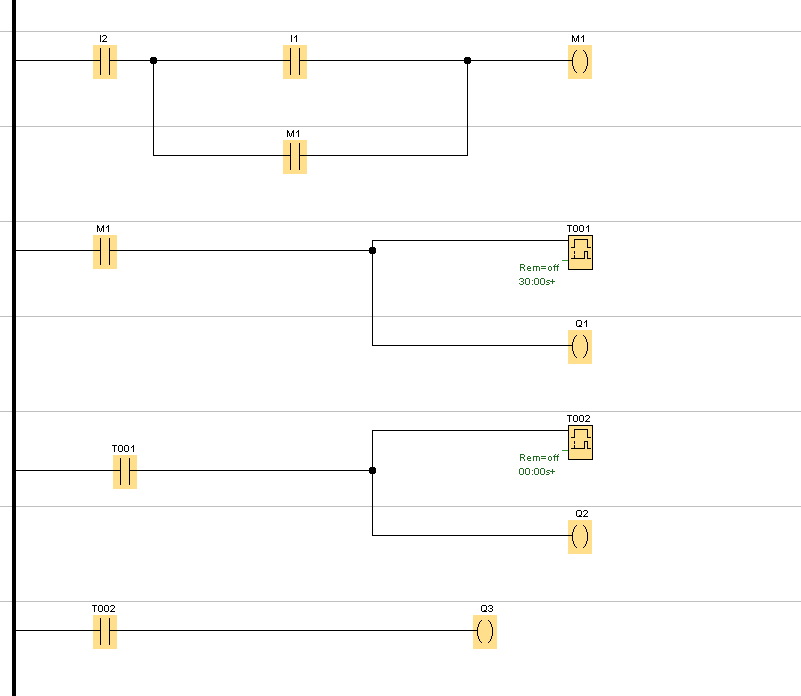
\includegraphics[width=0.92\textwidth]{rys/iteracja2.png}
    \caption{Iteracja 2 --- podtrzymanie na markerze M1}
    \label{fig:iter2}
\end{figure}

\subsection{Sygnały awarii napędów}

Wersja z markerem nadaje się już do sterowania załącz/wyłącz, ale nie reaguje na to, że któryś silnik wypadł z ruchu. Dołożyliśmy więc wejścia ze styków pomocniczych wyłączników silnikowych: I3 dla napędu 1, I4 dla napędu 2 i I5 dla napędu 3. W drabince stoją jako styki zanegowane w szeregu z cewką danego napędu. Pojawienie się awarii zdejmuje tylko ten napęd, którego dotyczy sygnał, a operator nadal gasi całość przyciskiem STOP.

\begin{figure}[H]
    \centering
    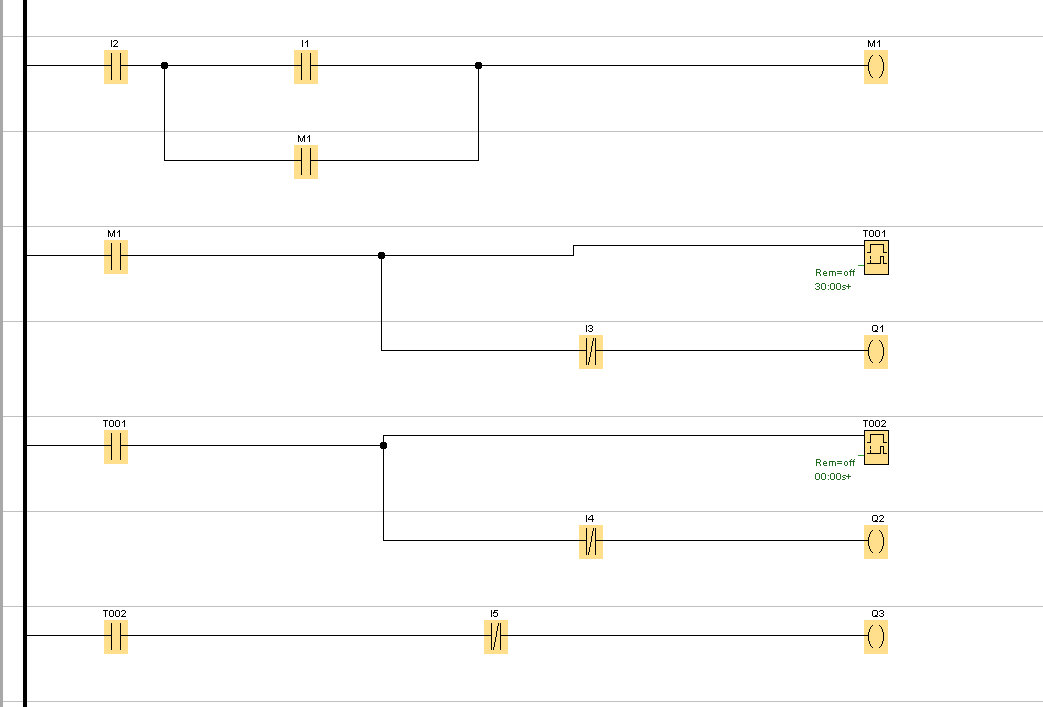
\includegraphics[width=0.92\textwidth]{rys/iteracja3.png}
    \caption{Iteracja 3 --- tory awarii I3, I4 i I5}
    \label{fig:iter3}
\end{figure}

\subsection{Symulowana awaria}

Schemat w obecnej postaci nie jest odporny na awarie. Jeżeli pierwszy podajnik uległby awarii, drugi oraz trzeci nadal by pracowały, bo nie ma warunku, który zależałby od Q1.

\begin{figure}[H]
    \centering
    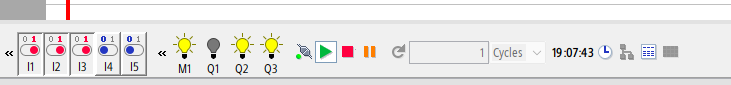
\includegraphics[width=0.92\textwidth]{rys/awaria.png}
    \caption{Symulowana awaria pierwszego podajnika}
    \label{fig:awaria}
\end{figure}